\chapter{Cubo content management system}
\label{chap:CuboCMS}

Il sistema per la gestione dei contenuti Cubo, rientra all'interno della categoria dei CMS proprietari e rappresenta una valida soluzione per lo sviluppo e la realizzazione di un sito web.\hfill \break
Lo strumento è stato sviluppato facendo fede a dei concetti cardine, ovvero flessibilità, modularità, scalabilità, accessibilità in termini d'uso e semplicità per quanto ne riguarda l'interazione da parte del cliente mediante l'utilizzo di strutture ad-hoc per la gestione delle pagine.\hfill \break
Seguirà un'analisi dei linguaggi e degli strumenti utilizzati, susseguita da supervisione globale all'interno della quale verrà analizzato il workflow in merito alla stesura e allo sviluppo del prodotto richiesto dal cliente.
\clearpage
\section{Linguaggi di programmazione}
Il linguaggio di programmazione[1] è un linguaggio formale che specifica un insieme di istruzioni utilizzate per produrre dati in uscita in merito al controllo del comportamento di una macchina formale (tipicamente, un computer) attraverso la stesura in fase di programmazione del codice sorgente, un particolare tipo di testo che definisce il flusso di esecuzione delle operazioni che devono essere eseguite.\hfill \break
Nella produzione di un CMS vengono impiegati linguaggi differenti, scelta dovuta all'eterogeneità che di base si vuole mettere a disposizione dell'utente, come ad esempio la parte grafica a discapito della zona adibito al coordinamento dei contenuti che di per se presenta una struttura logica completamente differente in relazione alla gestione delle risorse, delle strutture dati e dell'utilizzo delle espressioni.
\subsection{Sviluppo back-end}
Il back-end rappresenta la parte del codice che elabora i dati e con la quale l'utente interagisce indirettamente. Di norma, non è presente all'interno di siti web statici (ovvero con contenuti non modificabili).
Dal punto di vista della programmazione ed in riferimento alla sezione d'interesse, la parte di back-end è stata sviluppata mediante l'utilizzo dei seguenti linguaggi:
\begin{itemize}
    \item \textbf{Python}: linguaggio di programmazione ad alto livello multi-paradigma, orientato agli oggetti ed adatto allo sviluppo di applicazioni distribuite. Tra le varie caratteristiche emergono l'utilizzo di variabili non tipizzate, l'indentazione per la sintassi specifica, capacità di overloading e la presenza di un ricco assortimento di tipi, funzioni e librerie standard.
    \item \textbf{JavaScript}: linguaggio di programmazione orientato agli oggetti e agli eventi nato nel 1995 per essere utilizzato nello sviluppo lato client (nel contesto web front-end) ed in seguito esteso anche al lato server. Viene sostanzialmente utilizzato come linguaggio integrato secondo diversi framework che ne consentano l'impiego server-side per la generazione di applicazioni che devono rispondere a numerose richieste in modo rapido ed efficiente.
\end{itemize}
La scelta del voler utilizzare python come linguaggio principale ricade sulla semplicità in termini sintattici, i framework messi a disposizione sono meno frammentati ed incentrati in un impiego ben definito (e.g. Django per lo sviluppo web), sia per la flessibilità e la generalità negli ambienti di utilizzo, che risultano essere molteplici (Web development, Machine Learning ecc...).
\subsection{Sviluppo front-end}
Il front-end è quella parte che si occupa della gestione delle interazione con l'utente per la produzione di dati in ingresso (trattati ed elaborati successivamente in ottica back-end per la produzione in output degli stessi).\hfill \break
Come linguaggio di programmazione, è stato utilizzato \textbf{JavaScript} (discusso nella sezione 3.1.1) per lo sviluppo dello scripting integrato alla realizzazione di applicazioni web dinamiche. \hfill \break
In termini trasversali, sono stati adottati i seguenti linguaggi:
\begin{itemize}
    \item \textbf{HTML}: sviluppato nel 1990, l'Hypertext Markup Language è un linguaggio di markup a dominio pubblico
    rappresentante uno standard per la definizione dei documenti all'interno del World Wide Web.
    \item \textbf{CSS}: pubblicato per la prima volta verso il termine del 1996, il Cascading Style Sheet é un linguaggio utilizzato per la definizione e la formattazione in termini grafici dei documenti scritti in un linguaggio di markup (e.g HTML).
\end{itemize}

\section{Framework e strumenti utilizzati}
Nello sviluppo di un CMS o di un applicativo in generale, con il progredire del tempo, ha preso campo l'utilizzo dei framework, architetture logiche caratterizzate da un insieme di classi astratte correlate tra di esse che in fase d'implementazione, vanno ad inizializzare e a definire un'infrastruttura generale per permettere la semplificazione in merito all'operato del programmatore in fase di progettazione software. Il loro scopo è quello di far risparmiare allo sviluppatore la riscrittura del codice ed evitare il fenomeno della ridondanza favorendo la sinteticità del codice. I vantaggi dell'utilizzo di questo particolare tipo di costrutto sono l'ottimizzazione dei tempi, l'organizzazione del codice e la messa a punto di funzionalità specifiche per determinati tipi di esigenze.
Nella scelta del framework è importante valutare il tipo di applicazione e l'architettura desiderata, evitando di focalizzarsi unicamente sulle caratteristiche tecniche messe a disposizione.\hfill \break
Per il CMS cubo, sono stati adottati i seguenti quadri strutturali:
\begin{itemize}
    \item \textbf{Django}: Web framework open source per lo sviluppo di applicazioni web strutturato secondo il paradigma MVT (Model-View-Template).
    Il progetto venne sviluppato dalla Django Software Foundation e successivamente distribuito nel 2005, mediante licenza BSD (senza copyleft). Tra le varie funzionalità spiccano l'astrazione del database relazionale ad oggetti con supporto multi-piattaforma, un sistema di template basato su tag ereditari ed un sistema per la gestione degli utenti con autenticazione mediante applicazione web.
    \item \textbf{Vue.js}: Framework JavaScript open source per la creazione di interfacce utente e single-page applications. È stato creato da Evan You, ex dipendente Google, che lo ha versionato e distribuito nel 2014. Offre un'ottima adattabilità associata al concetto della scalabilità, fattori chiave nello sviluppo delle applicazioni web.
\end{itemize}

\subsection{API Web}
Per semplificare ulteriormente l'operato del programmatore, sono state utilizzate le API (acronimo di Application Programming Interface)[2], un set di definizioni e protocolli con i quali vengono realizzati e integrati software applicativi. L'obiettivo è quello di semplificare la possibilità di dialogo tra un'applicazione e l'altra garantendo allo stesso tempo amministrazione e flessibilità.
Vengono largamente utilizzate per l'accoppiamento con software di terze parti, favorendo la migrazione verso lo sviluppo di un modello d'architettura orientata ai servizi (SOA, Service Oriented Architecture). \hfill \break
Per l'accesso ai web services, sono state integrate le API RESTful, strutturate secondo i vincoli architettonici REST (acronimo di REpresentional State Transfer).

\begin{figure}[ht!]
    \centering
    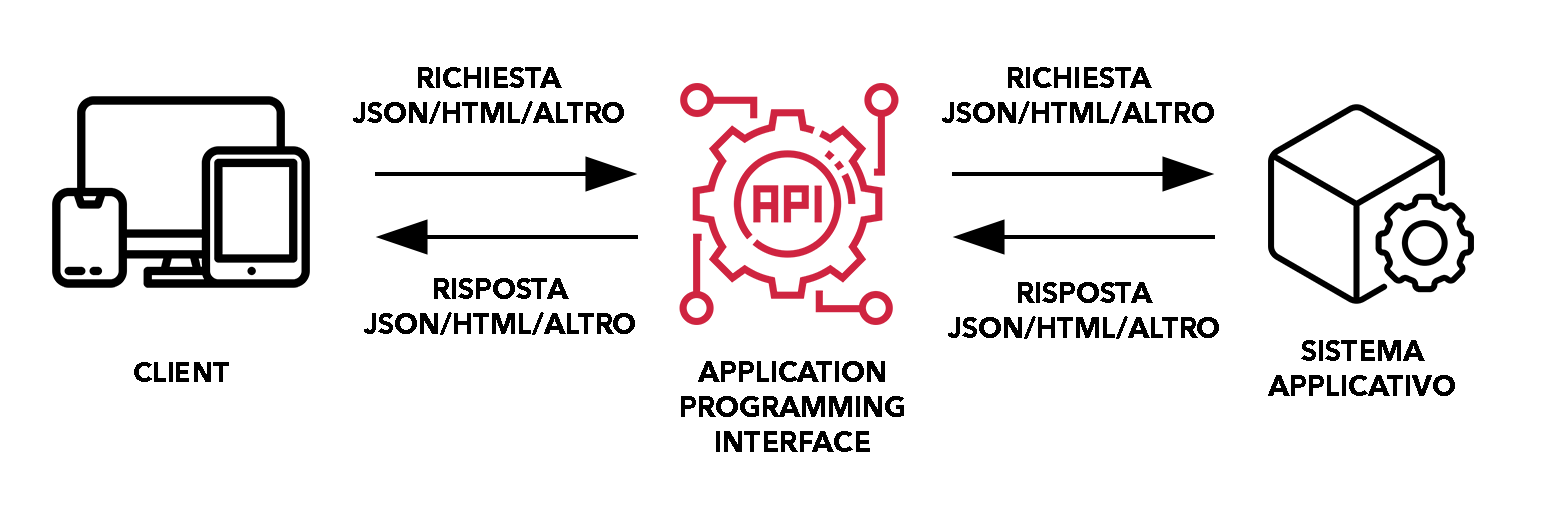
\includegraphics[width=150mm]{images/API.png}
    \caption{Rappresentazione concettuale di un'API\label{overflow}}
\end{figure}

Quando il client inoltra una determinata richiesta, l'API trasferisce al richiedente (o all'endpoint) uno stato rappresentativo della risorsa che, tramite protocollo HTTP, viene consegnata in uno dei diversi formati disponibili (e.g. JSON, HTML, PHP, testo semplice).
\clearpage
Le API sono definibili RESTful se rispettano i seguenti sei vincoli:
\begin{itemize}
    \item Un'architettura client-server composta da client, server e risorse, con richieste gestite tramite HTTP.
    \item Una comunicazione client-server stateless, che quindi non prevede la memorizzazione delle informazioni del client tra le richieste GET: ogni richiesta è distinta e non connessa.
    \item Dati memorizzabili nella cache che ottimizzano le interazioni client-server.
    \item Un'interfaccia uniforme per i componenti, in modo che le informazioni vengano trasferite in una forma standard.
    \item Un sistema su più livelli che organizza ogni tipo di server che si occupa di recuperare le informazioni richieste in gerarchie, invisibile al client.
    \item Codice on demand (facoltativo): la capacità di inviare codice eseguibile dal server al client quando richiesto, estendendo la funzionalità del client.
\end{itemize}

La scelta per quanto ne riguarda l'utilizzo delle API in questione è da associare al REST che mette a disposizione i dati sotto forma di risorsa anziché di servizio ed il fatto che vada ad integrare i verbi HTTP come GET, POST, PUT e DELETE, necessari per comunicare al server cosa fare con i dati identificati dall'URL di una specifica risorsa.
\clearpage

\section{Struttura ed architettura} 
All'interno della seguente sezione viene analizzata la struttura e l'architettura del content management system Cubo. 
Nello specifico, vengono trattati gli elementi base sui quali si erge il sistema proprietario con un particolare riferimento all'applicazione degli strumenti e delle tecnologie citate precedentemente, l'impatto dell'implementazione circa eventuali personalizzazioni richieste dal cliente e il workflow dell'interazione e della gestione dei contenuti.

\begin{figure}[ht!]
    \centering
    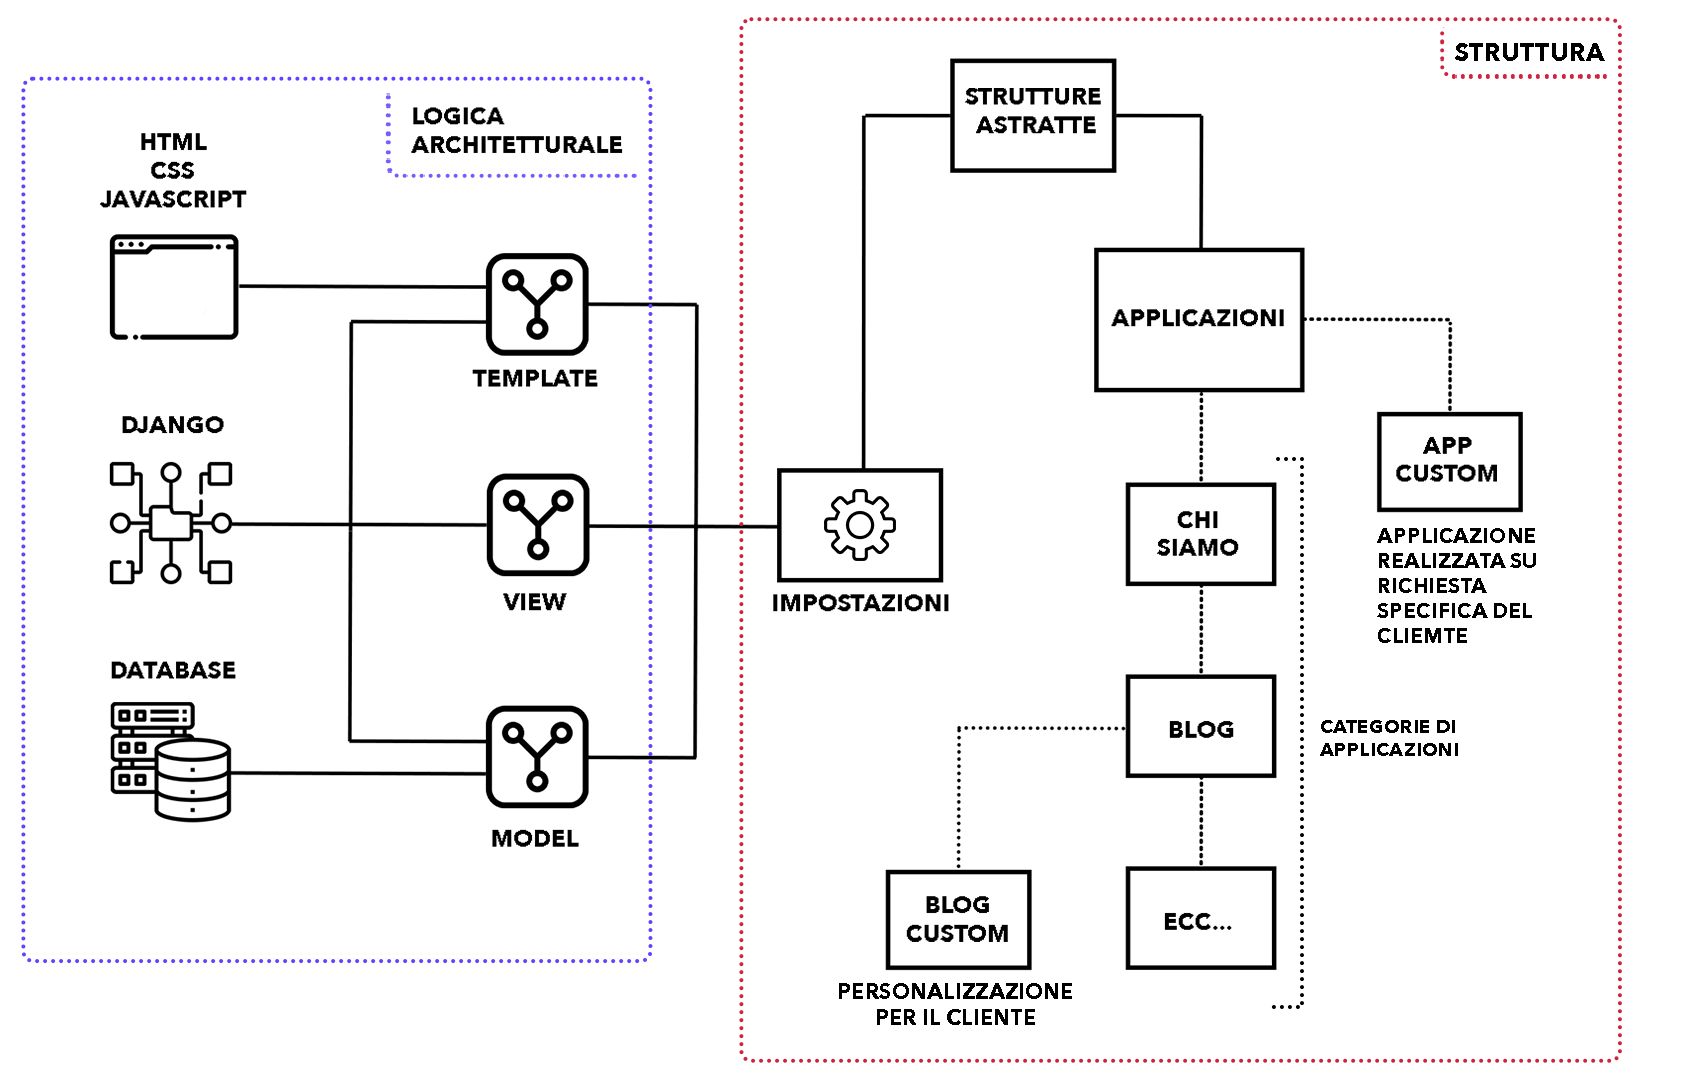
\includegraphics[width=155mm]{images/Cubo CMS Struttura.png}
    \caption{Cubo CMS, struttura ed architettura logica \label{overflow}}
\end{figure}
\clearpage
\subsection{Django e il paradigma MVT}
L'architettura del framework Django (introdotto nel capitolo 3.2) segue i criteri del paradigma Model-View-Template (MVT - Modello, Vista e Template), un pattern utilizzato per lo sviluppo delle applicazioni e delle interfacce Web strutturato secondo i seguenti concetti:
\begin{itemize}
    \item \textbf{Modello}: Un livello astratto dove viene generata e gestita l'infrastruttura per la manipolazione dei dati. All'interno sono presenti delle classi per la rappresentazione delle tabelle contenute all'interno del database e per l'utilizzo delle operazioni CRUD (CREATE, READ, UPDATE, DELETE) in fase d'interazione coi dati.
    \item \textbf{Vista}: Strato incaricato dell'elaborazione delle richieste effettuate da parte degli utenti. Le funzioni che lo stesso mette a disposizione, vengono utilizzate per amministrare le interazioni, estrarre i dati dal database, elaborarli e fornire una risposta rappresentativa attraverso il template.
    \item \textbf{Template}: identificabile attraverso un file utilizzato per la rappresentazione dei dati processati all'interno della vista di riferimento. Presenta una sintassi semplice ed al suo interno avviene la conversione delle informazioni in elementi associabili al linguaggio HTML.
\end{itemize}

\clearpage
\begin{figure}[ht!]
    \centering
    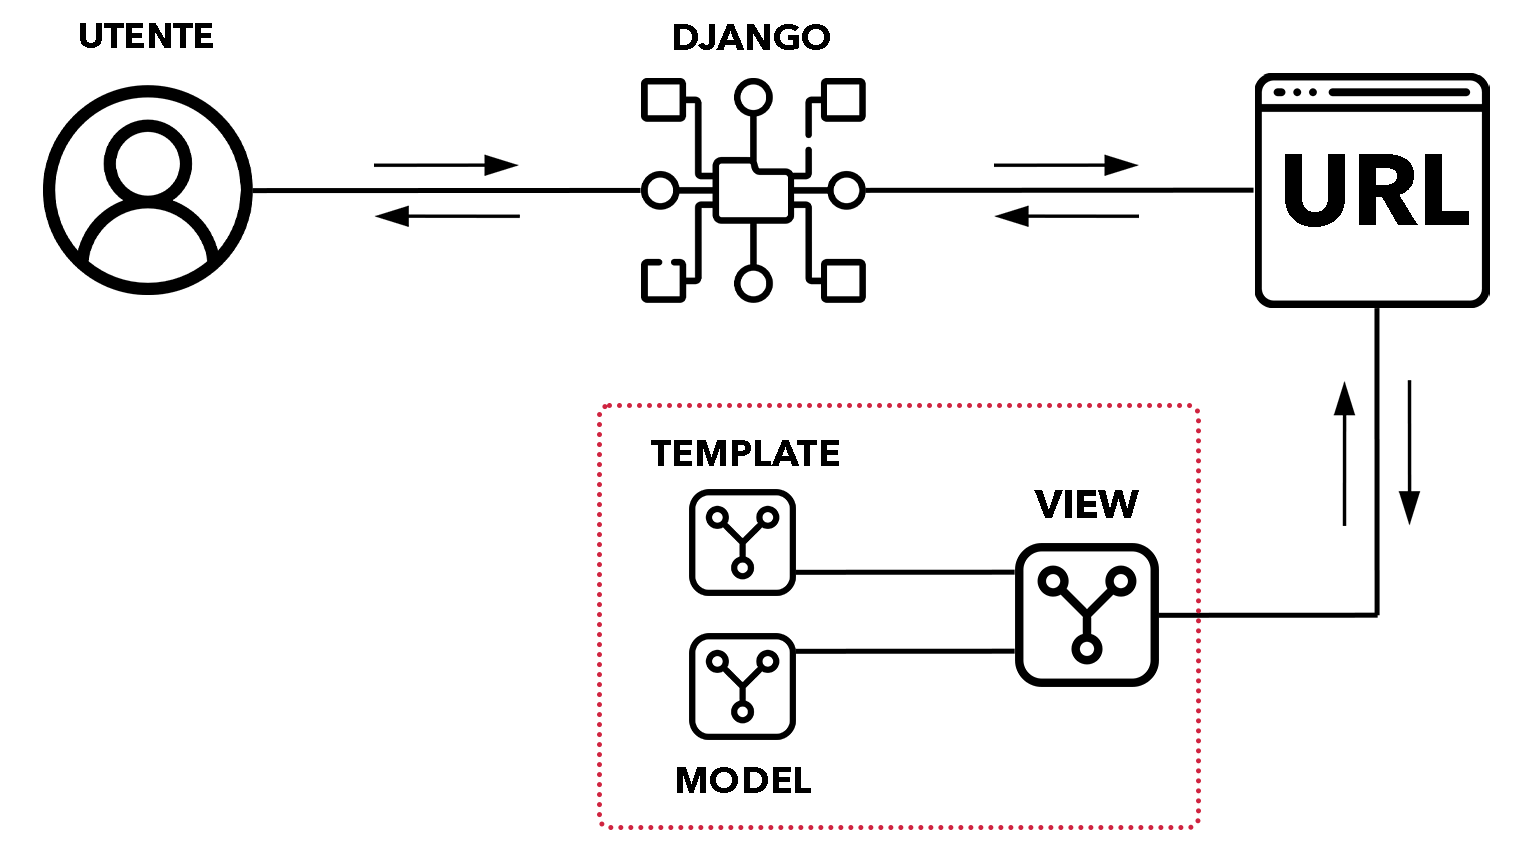
\includegraphics[width=120mm]{images/Paradigma MVT.png}
    \caption{Workflow del paradigma MVT \label{overflow}}
\end{figure}

L'utente effettua una richiesta che viene automaticamente gestita dal framework. Quest'ultimo analizza la disponibilità delle risorse tramite l'URL (Uniform Resource Locator)[3], una sequenza di caratteri che identifica univocamente l'indirizzo di una risorsa. In caso la mappatura dovesse dare esito positivo, si procede con l'utilizzo della funzione per il richiamo della vista che andrà ad interagire con il modello ed il template di riferimento. Una volta generato, il template viene incapsulato all'interno di una risposta presa in carico da Django inviata successivamente all'utente, libero di poterne interagire.

\clearpage

\subsection{Configurazione delle impostazioni}
Le impostazioni sono alla base della predisposizione per quanto ne riguarda l'utilizzo di tutti gli elementi d'interesse presenti all'interno del progetto. \hfill \break
In termini caratteristici, al loro interno troviamo:
\begin{itemize}
    \item \textbf{Ambienti Diversificati}: Ogni ambiente presenta impostazioni e configurazioni specifiche per il coordinamento dei servizi e/o delle strutture.
    \item \textbf{Dati sensibili}: Password del Database, token per API di terze parti, credenziali per l'accesso a determinati servizi.
\end{itemize}

È necessario far uso di una pratica che permetta l'eliminazione dell'errore umano in fase di pianificazione (uno sviluppatore potrebbe andare ad integrare un API e non riuscire ad aggiungere delle impostazioni specifiche per l'utilizzo della stessa all'interno del progetto, andandone a compromettere l'operato su larga scala). 
Dal punto di vista pratico, è stato utilizzato un approccio procedurale: in un primo momento si vanno a definire le applicazioni da implementare all'interno del sito in fase di sviluppo susseguiti dalla definizione delle lingue supportate (su specifica richiesta del cliente), i vari percorsi per poter accedere ai template, ai contenuti grafici e a quelli statici. 
In seguito, si passa agli strumenti per il debug e l'associazione con il database d'interesse (che deve essere già stato inizializzato a priori). 
Si procede con l'instaurazione della Sitemap, un particolare tipo di file contente tutti gli URL presenti all'interno del sito. Il suo obiettivo è agevolare la navigazione client-side migliorando l'impatto nel contesto della scansione e dell'indicizzazione web.
Infine, si va ad ultimare il tutto attraverso la configurazione della WSGI (Web Server Gateway Interface)[4], un protocollo di trasmissione che stabilisce e descrive comunicazioni ed interazioni tra server ed applicazioni web scritte nel linguaggio Python. Il protocollo specifica come i server si facciano carico delle richieste provenienti dai browser/client ed inoltrino le informazioni richieste alle relative applicazioni.


\subsection{Applicazioni}
Il CMS Cubo mette a disposizione diverse applicazioni strutturate secondo l'architettura client-server e focalizzate nell'offrire determinati servizi all'utente client in fase d'interazione sulla base logica del paradigma MVT (discusso precedentemente).\hfill \break
Ogni singola applicazione si articola di tutti gli elementi necessari per un corretto funzionamento, ovvero modelli, viste, template ed URL specifici. \hfill \break
Lo sviluppo avviene mediante l'utilizzo dei modelli astratti, fondamentali in ottica di risparmio e minimizzazione del codice.
All'interno del progetto è presente una particolare applicazione, denominata \textit{Core}, nella quale presenzia tutta la componentistica necessaria per poter mettere in pratica l'approccio nella sua concezione astratta.
Nell'ipotetico esempio della generazione di un \textit{modello} per una determinata applicazione, si procederà con l'importazione del modello astratto \textit{StandardPageMetaModel} (specifico per i modelli) e l'inizializzazione della classe con i relativi \textit{meta-dati} (rappresentati un'insieme di informazioni necessari per una corretta gestione e conservazione nel tempo delle risorse). \hfill \break
\lstinputlisting[firstline=1, lastline=9, caption={Principio dell'eredità applicato al modello}]{code/ExampleModel MVT.py}
Il workflow appena analizzato, utilizza il principio dell'ereditarietà e viene iterato anche nel processo per la generazione delle viste e dei template.\hfill\break
Nel caso dei template si fa utilizzo del file \textit{\_base.html}, che definisce la struttura sulla quale proseguiranno le operazioni di sviluppo front-end. \hfill \break
In ottica architetturale il template fa uso dello sviluppo a blocchi per poter far fede al concetto dell'ottimizzazione e della pulizia del codice. \hfill \break
I blocchi sono delimitati da dei tag che ne definiscono la struttura logico-gerarchica e durante la generazione del template di un'ipotetica applicazione, a seguito dell'importazione del file  \textit{\_base.html} al suo interno, prenderà campo la sovrascrittura dei blocchi di riferimento con successiva implementazione del codice HTML. \hfill \break
\lstinputlisting[firstline=1, lastline=13, caption={Struttura dei blocchi all'interno del \_base.html}]{code/_base.html}
\clearpage
L'ipotetico template dell'applicazione avrà di conseguenza ereditato l'aspetto e la logica sintattica del \textit{Core} template, pronto per essere personalizzato nel caso di una particolare richiesta da parte del cliente.
\lstinputlisting[firstline=1, lastline=5, caption={Sovrascrittura all'interno del template ereditario}]{code/_son.html}

\subsubsection{Modelli astratti}
In fase di programmazione, la gestione e l'ordine del codice sono fondamentali. L'utilizzo dei modelli astratti favorisce una pratica precisa, pulita ed ottimizzata per lo sviluppo del CMS.\hfill \break
Tali modelli, fanno uso del concetto della metamodellazione[5], strutturato sull'analisi, sulla costruzione e sullo sviluppo di strutture, regole, vincoli, modelli e teorie applicabili ed utilizzabili per la modellazione di classi predefinite di problemi.
Mentre il modello rappresenta un'astrazione dell'idea di una determinata entità, il meta-modello si identifica in un ulteriore astrazione dello stesso e con una definizione più approfondita delle strutture e dei vari elementi al suo interno. \hfill \break
Il modello \textit{StandardPageMetaModel} rappresenta un caso concreto della messa in pratica di questo tipologia d'approccio.
Per unificare la metodologia, sono state sviluppate anche innumerevoli classi astratte secondo l'immagine dell'ereditarietà multipla[6], in cui una classe può ereditare funzionalità e caratteristiche da più di una classe base. \hfill \break
All'interno delle viste adibite al servizio amministrativo troviamo classi come \textit{BaseCreate} e \textit{BaseUpdate}, incaricate della gestione form-view, che una volta concretizzate (nel contesto dello sviluppo di un'applicazione), estendono tutte le funzionalità a loro disposizione con una successiva sovrascrittura degli attributi (specifici) d'interesse per la classe appena inizializzata.


\subsection{Database}
Il database è un sistema informatico attuo alla memorizzazione permanente dei dati ed in senso tecnico, può essere definito com un archivio strutturato per la conservazione e il mantenimento dei dati. Il framework Django, utilizza i modelli per interagire con database e sempre secondo il concetto della programmazione orientata agli oggetti. \hfill \break
Il modello, pertanto, si identifica nella forma di un oggetto caratterizzato da determinate proprietà. All'interno del database, quest'ultimo assume l'aspetto di una tabella, a sua volta popolata da righe e colonne, che ne rappresentano rispettivamente le istanze e gli attributi. In seguito, tra le varie tabelle, vengono definiti i vincoli e le associazioni alla base della logica relazionale adottata.
Il modelli e le tabelle costituiscono un dualismo che deve procedere in maniera sincrona per poter garantire un mantenimento efficiente delle risorse e dell'infrastruttura adibita all'interrogazioni del database.
Django utilizza le migrazioni per prorogare ed apportare eventuali modifiche effettuate sui modelli al database con una diretta e conseguente generazione del file di migrazione, un particolare tipo di documento all'interno del quale viene tenuta traccia di tutte le variazioni effettuate dalla suddetta procedura.

\clearpage

\subsection{Console di amministrazione}
Dopo aver ultimato tutte le strutture ed aver configurato in maniera specifica tutte le varie impostazioni, il sito si prepara ad essere popolato secondo i parametri e i contenuti d'interesse. Cubo CMS predispone un pratico pannello di amministrazione all'interno del quale è possibile andare ad inserire, gestire e supervisionare tutti gli elementi che si reputano opportuni. La dashboard è stata strutturata in maniera da predisporre un utilizzo facile ed intuitivo per l'utente amministratore. Ogni applicazione, all'interno del pannello, presenta una sezione dedicata dove è possibile andarne a modificare ogni aspetto correlato al contesto amministrativo della stessa in maniera indipendente nel rispetto delle altre applicazioni installate.

\begin{figure}[ht!]
    \centering
    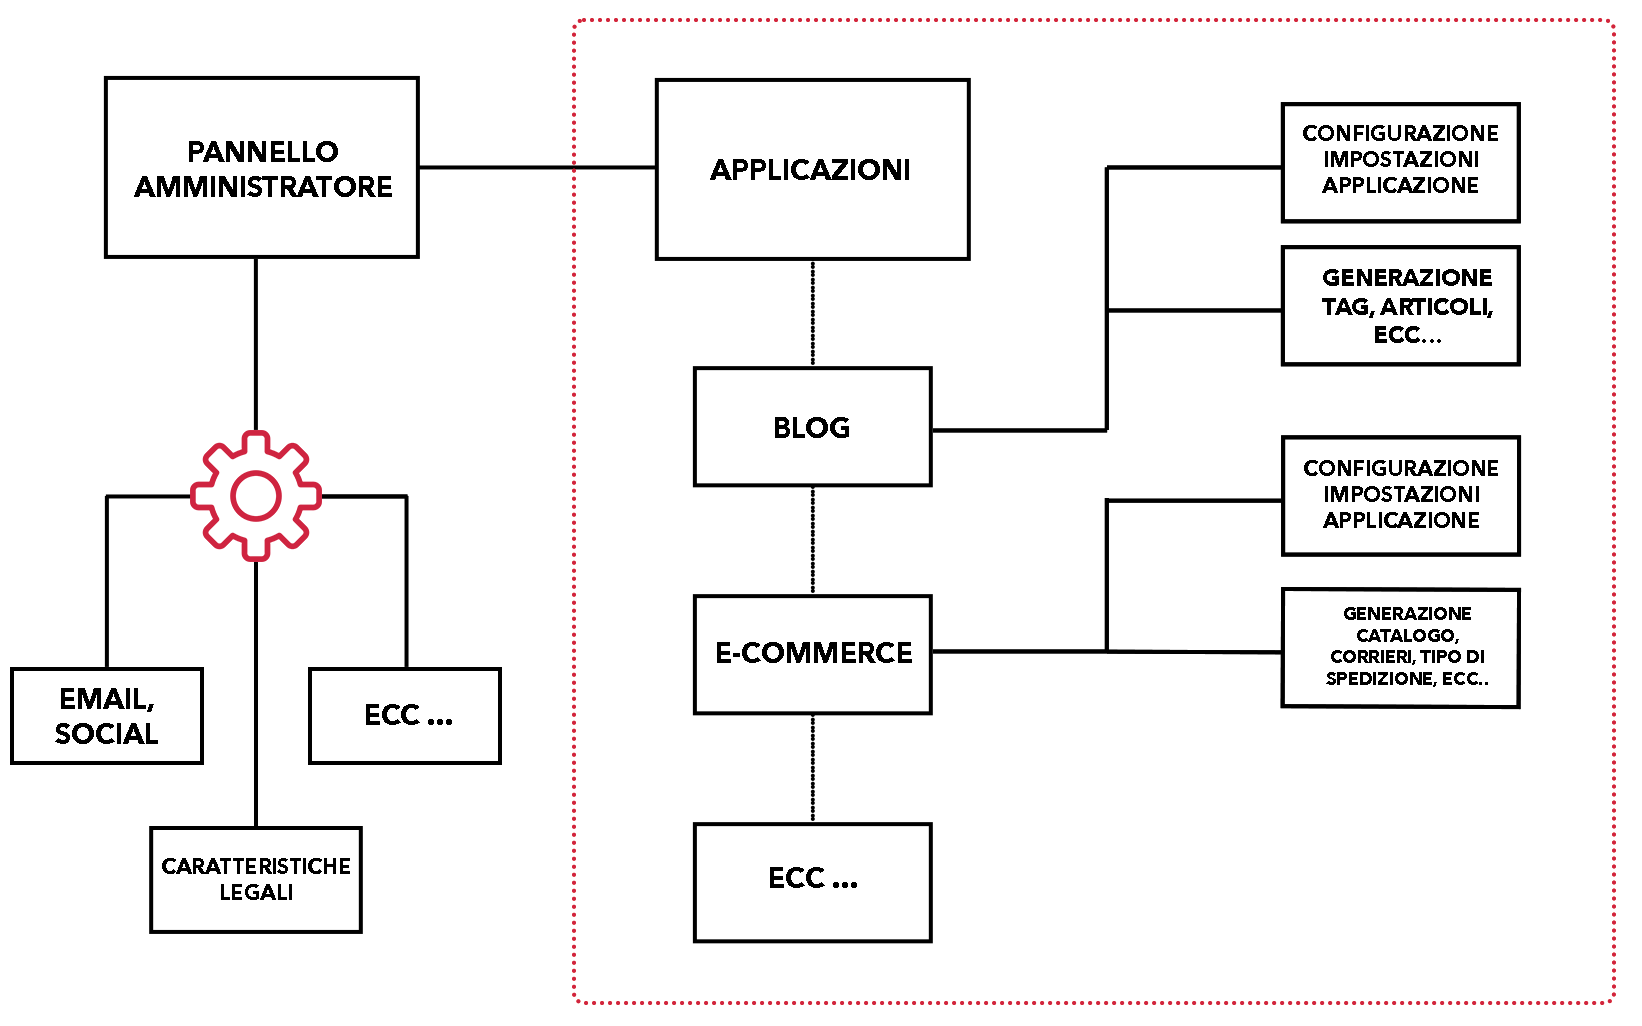
\includegraphics[width=140mm]{images/Struttura Console amministrazione.png}
    \caption{Struttura della console amministrativa\label{overflow}}
\end{figure}

\subsubsection{Blocchi per la personalizzazione}
Il sistema per la gestione dei contenuti deve adattarsi alle richieste e alle esigenze del cliente. A tal proposito, la personalizzazione del sito riveste un ruolo fondamentale e lo strumento mette a disposizione diverse funzionalità per poter procedere in questa direzione. In termini tecnici, come molti altri CMS, anche Cubo fornisce dei blocchi, ovvero dei moduli preconfigurati che possono essere utilizzati per la costruzione del sito nelle sue componentistiche (come ad esempio per le testate, i footer, le sezioni dedicate ad un determinato contenuto, la modifica del logo del sito ecc...).\hfill \break
L'utilizzo dei blocchi estende il concetto della modularità e della flessibilità. Attraverso i seguenti costrutti, l'amministratore può modificare a suo piacimento l'estetica e i contenuti presenti all'interno delle differenti pagine, senza la necessità di particolari conoscenze tecniche. Allo stesso tempo, l'implementazione di questo tipo di approccio ha uniformato ulteriormente le pratiche in fase di programmazione, evitando costanti modifiche sulla base della particolari commesse da parte del cliente.
